\chapter{Design Sensitivity Analysis}
In this chapter, the concept behind discrete and continuum sensitivity formulation is discussed and the general approach for deriving the sensitivity equations is presented. The two sensitivity analysis techniques are applied to a heat transfer benchmark problem where the sensitivity of response to the shape of the domain is calculated. This problem is also used in the next chapter for implementation of different immersed boundary methods. The difference between local and total formulation of the sensitivity response is discussed and finally the independence of continuum sensitivity formulation to discretization method is proven. This enables use to reuse the solver of governing equation to calculate the sensitivity response. This is typically not possible for discrete sensitivity formulation.

% ======================================================================================
\section{General formulation}
The general computational domain is defined as shown in Figure \ref{fig:C2_continuumDomain}. The response variable on this domain can be from the fluid, i.e. pressure or velocity, or the solid, i.e. displacements. Nevertheless, the response is calculated using a governing equation subject to boundary conditions. In this work, the governing equation and boundary conditions are represented in the functional form as shown in Equation \eqref{eq:C2_governingEquationAndBC}.

\begin{subequations}
\begin{gather}
	\mathbf{A}(\mathbf{u}, t; \mathbf{b}) = \mathbf{f}(\mathbf{x}, t; \mathbf{b})
	\quad \text{on} \quad \Omega
	\\
	\mathbf{B}(\mathbf{u}, t; \mathbf{b}) = \mathbf{g}(\mathbf{x}, t; \mathbf{b})	
	\quad \text{on} \quad \Gamma
\end{gather}\label{eq:C2_governingEquationAndBC}
\end{subequations}

where $\mathbf{A}$ is the governing equation such as Navier-Stokes equations or elastic equations and $\mathbf{B}$ is the boundary condition definition. $\mathbf{u}$ is the response variable such as displacement or pressure. $t$ is time, $\mathbf{b}$ is the design variable such as shape or size, and $\mathbf{x}$ is the spatial coordinate. $\mathbf{f}$ and $\mathbf{g}$ is the value of governing equation and boundary condition. The sensitivity of response variable with respect to $i$-th design variable $b_i$, $\partial \mathbf{u}/\partial b_i$, can be calculate using some sensitivity analysis technique. This is done in the following sections.

The total sensitivity of response variable, $\mathbf{u}$ with respect to the $i$-th design variable is written as

\begin{equation}\label{eq:C2_totalSensitivityDef}
	\frac{D \mathbf{u}}{D b_i} = 
	\frac{\partial \mathbf{u}}{\partial b_i} + 
	\frac{\partial \mathbf{u}}{\partial \mathbf{x}} \cdot
	\frac{\partial \mathbf{x}}{\partial b_i} 
\end{equation}

The total derivative is known as material derivative in continuum mechanics \cite{mase2009continuum}. This total sensitivity defines the change of response variable, $\mathbf{u}$, subjected to design variable and space dependent changes. The material derivative consists of the local derivative, $\partial \mathbf{u}/\partial b_i$, plus the convective term, $\partial \mathbf{u}/\partial \mathbf{x} \cdot \partial \mathbf{x}/\partial b_i$. The local derivative is the measure of change in the response variable due to change in the design parameter. Whereas, the convective term accounts for the movement of this point in space due to change in the design variable. This is specially applicable to shape sensitivity calculating where the change in design variable, will cause the material points to move \cite{cross2014local}. The convective term consists of two separate gradients: i) $\partial \mathbf{u} / \partial \mathbf{x}$ which represents the spatial gradient of the response variable in the domain, and ii) $\partial \mathbf{x} / \partial b_i$ which defines the sensitivity of the spatial domain with respect to the change in design variable. The later defines how the computational nodes moves as the design variable changes. The response variable spatial gradient term can be calculated using the analysis results, using finite difference approach or derivative of shape functions in FEA formulation. Calculation of domain sensitivity, $\partial \mathbf{x} / \partial b_i$, requires more attention.

A common approach to calculate the domain sensitivity, is to use the same techniques used to deform the body-conformal mesh in a CFD simulation. These methods are usually based on representing the computational grid as a system of springs that connected to each other at the nodes. This system can be modeled and solved using structural analysis techniques, where the sensitivities can be easily added to its formulation. This is effectively a shape sensitivity analysis for the structural analyses \cite{haftka1986structural}. This step can be removed from the analysis if the computational domain does not affected by design variable since $\partial x/\partial b$ is equal to zero for this case. This is removes the extra step of doing the structural shape sensitivity analysis for the mesh and also response variable gradient calculation. As mentioned in Chapter \ref{ch:introduction}, by using the immersed boundary method the mesh definition is decoupled from the boundary shape. Therefore, domain sensitivity is equal to zero \cite{gobal2014continuum}. This is one of the reasons to use the immersed boundary calculation since it reduces the cost of the simulation. This is discussed in more details in Chapter \ref{ch:immersedBoundary}.

% ======================================================================================
\section{Benchmark case}
To compare the discrete and continuum sensitivity analysis we chose the one-dimensional heat transfer analysis in a rod. The temperature in governing by the Laplace equation as shown in Equation \eqref{eq:C2_laplaceEquation}.

\begin{equation}\label{eq:C2_laplaceEquation}
	\frac{\partial^2 T}{\partial x^2} = 0
\end{equation}

where $T$ is the temperature and $x$ is spatial variable. The boundary conditions are defined as constant temperatures at the two ends of the domain as shown in Figure \ref{fig:C2_benchmarkCase}. The length of domain is selected as $L$.

\begin{figure}[h]
	\centering
	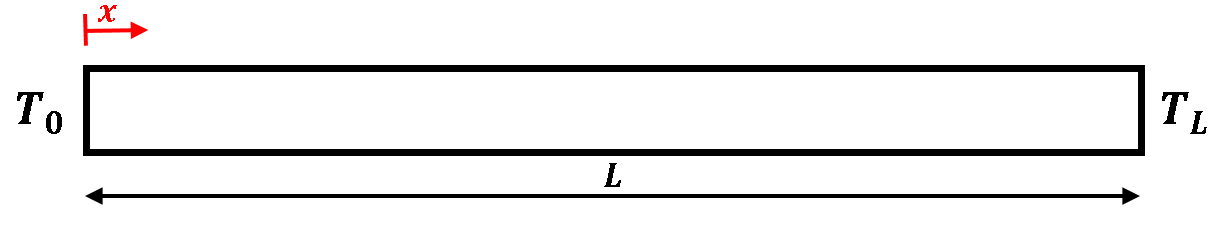
\includegraphics[width=14.00cm]{Chapter_2/figure/benchmark_case.png}
	\caption{One dimensional domain with heat conduction.}
	\label{fig:C2_benchmarkCase}
\end{figure}

The analytical solution of Equation \eqref{eq:C2_laplaceEquation} can be written as follows

\begin{equation}\label{eq:C2_benchmarkCaseAnalyticalSolution}
	T = \frac{T_L - T_0}{L} x + T_0
\end{equation}

The analytical sensitivity of the temperature with respect to beam's length can be calculated by differentiating Equation \eqref{eq:C2_benchmarkCaseAnalyticalSolution} with respect to $L$.

\begin{equation}
	\frac{\partial T}{\partial L} = -\frac{T_L - T_0}{L^2} x
\end{equation}

Since the analytical derivatives are known, we can compare it to the discrete and continuous sensitivity results.

% ======================================================================================
\section{Discrete sensitivity formulation}
To formulate the discrete sensitivity equation, we start by discretizing the governing equation \eqref{eq:C2_laplaceEquation} using finite difference method. It should be noted that the finite difference is used for discretization of continuum governing equation and not sensitivity calculation. The design variable effects the shape of the domain which is the distance between the nodes in the discrete manner. Therefore, for the sake of sensitivity analysis it is required to keep the nodal distances in the discretized solution as well. We use 6 nodes to discretize the domain as shown in Figure \ref{fig:C2_discretizedDomain}.

\begin{figure}[h]
	\centering
	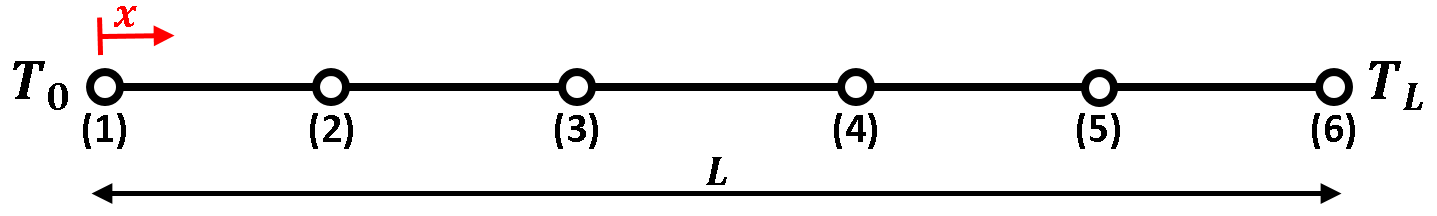
\includegraphics[width=14.00cm]{Chapter_2/figure/benchmark_case_computational_domain.png}
	\caption{One dimensional computational domain for heat conduction.}
	\label{fig:C2_discretizedDomain}
\end{figure}

To discretize Equation \eqref{eq:C2_laplaceEquation}, the first step is to approximate the second derivative. This is done by writing the Taylor series expansion at at arbitrary location $x_i$.

\begin{equation*}
	T(x) = 
	T(x_0) + 
	\frac{\partial T}{\partial x} \bigg|_{x_i} (x - x_i) + 
	\frac{\partial^2 T}{\partial x^2} \bigg|_{x_i} (x - x_i)^2 + 
	\mathcal{H} . \mathcal{O} . \mathcal{T}
\end{equation*}

To approximate the second derivative at the arbitrary node $x_i$ using central method we need to use the neighbouring nodes. The second order approximation for the second order derivative of central difference method is shown in Equation \eqref{eq:C2_finiteDifferenceSchemes}. The discretized equations are differentiated with respect to shape design variable. This requires the nodal distances to be included in the discretized equations. To maintain the generality, we assume that distance of node $T_i$ to $T_{i+1}$ is $\Delta_i$ and the distance of node $T_i$ to $T_{i-1}$ is $\Delta_{i-1}$.

\begin{equation}\label{eq:C2_finiteDifferenceSchemes}
	\frac{\partial^2 T}{\partial x^2} = 
	\frac{T_{i-1} \Delta_{iL} - 
	      T_{i} (\Delta_{iL} + \Delta_{iR}) + 
	      T_{i+1} \Delta_{iR}}
	     {\dfrac{1}{2} \left[ \Delta_{iL} \Delta_{iR}^2 + 
	                         \Delta_{iL}^2 \Delta_{iR} \right]}
\end{equation}

The approximation of the second derivative in Equation \eqref{eq:C2_laplaceEquation} is done using definitions in Equation \eqref{eq:C2_finiteDifferenceSchemes} for each node excluding the boundary nodes. As mentioned in the previous section, the nodal values at boundary nodes, $(1)$ and $(2)$ are known. The discretized governing equations is written in the matrix form as shown in Equation \eqref{eq:C2_laplaceEquationMatrixForm}.

\begin{equation}\label{eq:C2_laplaceEquationMatrixForm}
	\begin{bmatrix}
		\frac{-2}{\Delta_{2L} \Delta_{2R}} &
		\frac{2}{\Delta_{2L} \Delta_{2R} + \Delta_{2L}^2} &
		0 &
		0 &
		\\
		\frac{2}{\Delta_{3R}^2 + \Delta_{3L} \Delta_{3R}} & 
		\frac{-2}{\Delta_{3L} \Delta_{3R}} &
		\frac{2}{\Delta_{3L} \Delta_{3R} + \Delta_{3L}^2} &
		0
		\\
		0 &
		\frac{2}{\Delta_{4R}^2 + \Delta_{4L} \Delta_{4R}} & 
		\frac{-2}{\Delta_{4L} \Delta_{4R}} &
		\frac{2}{\Delta_{4L} \Delta_{4R} + \Delta_{4L}^2} &
		\\
		0 &
		0 &
		\frac{2}{\Delta_{5R}^2 + \Delta_{5L} \Delta_{5R}} & 
		\frac{-2}{\Delta_{5L} \Delta_{5R}}
	\end{bmatrix}
	\begin{bmatrix}
		T_2 \\
		T_3 \\
		T_4 \\
		T_5
	\end{bmatrix}
	=
	-\begin{bmatrix}
	 	\frac{2T_1}{\Delta_{2R}^2 + \Delta_{2L} \Delta_{2R}} \\
 		0 \\
		0 \\
		\frac{2T_6}{\Delta_{5L} \Delta_{5R} + \Delta_{5L}^2}
	\end{bmatrix}
\end{equation}

To verify the discretization process, we compare the analytical solution of this problem with the result of Equation \eqref{eq:C2_laplaceEquationMatrixForm} in Figure \ref{fig:C2_verificationOfSolver}. For this problem we choose $T_1 = 0$, $T_6 = 1$, and $L = 1$.  As shown in this figure, the discrete and continuum results match very well.

\begin{figure}[h]
	\centering
	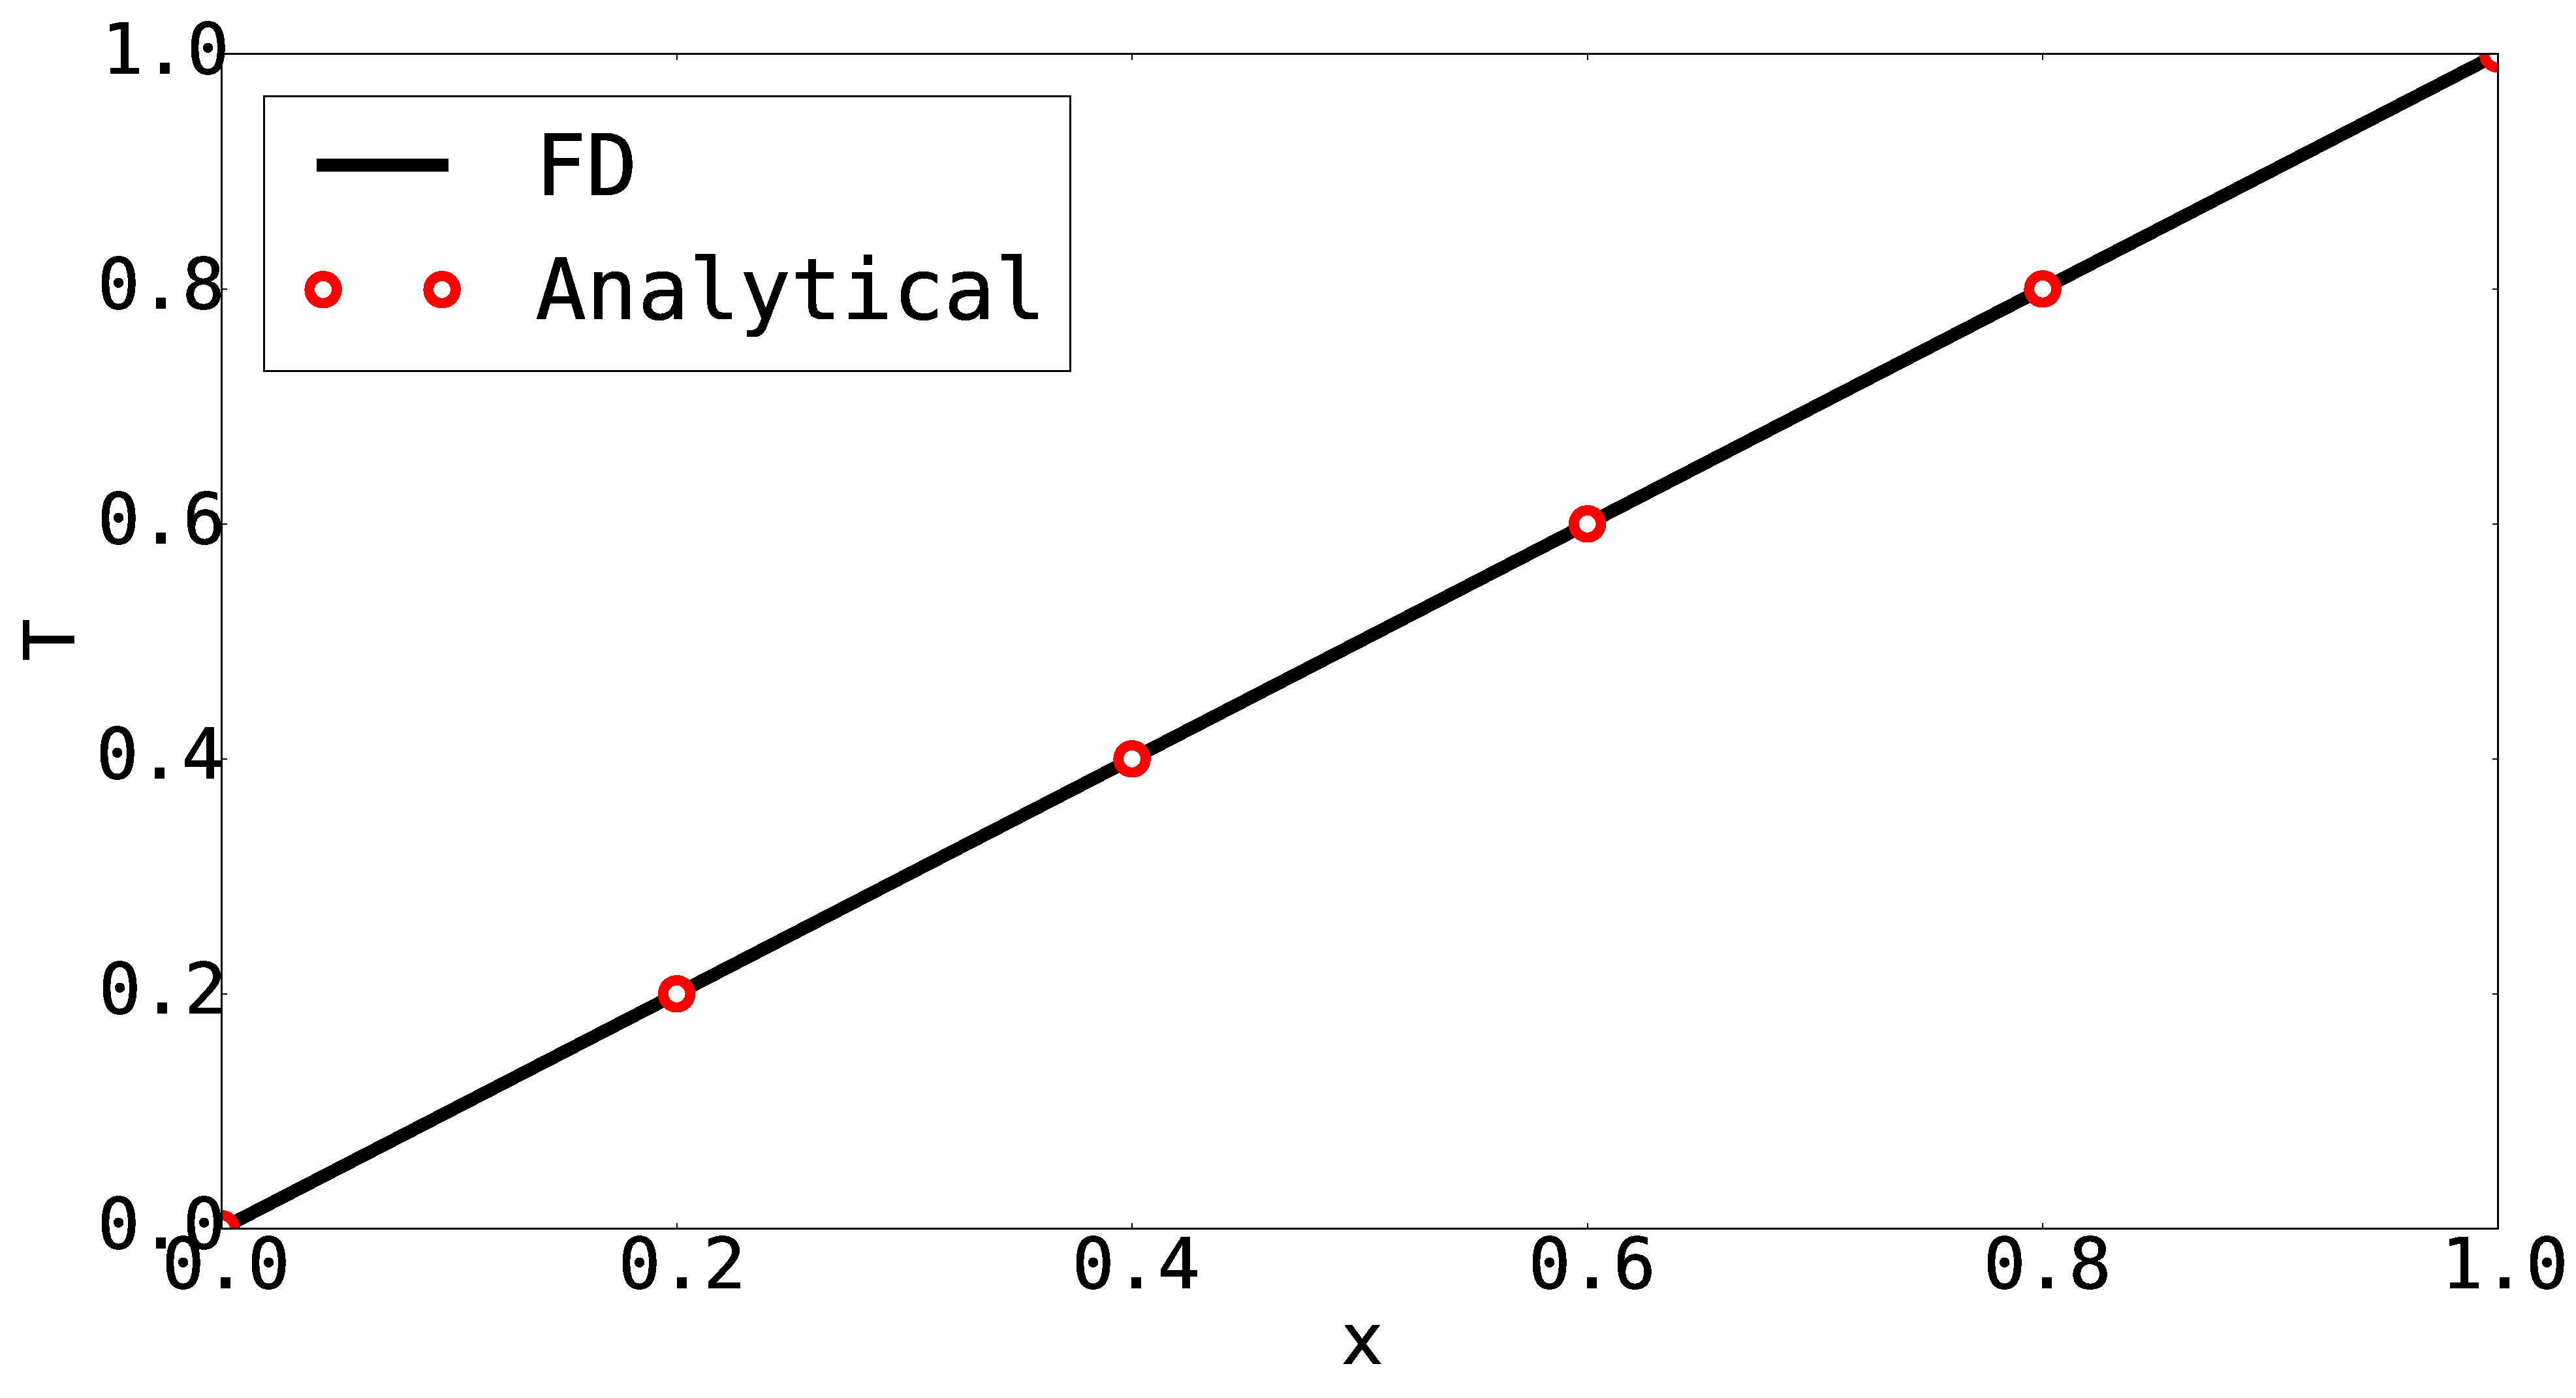
\includegraphics[height=9.00cm]{Chapter_2/figure/finitedifference_vs_analytical.eps}
	\caption{Comparison between the analytical and finite difference solution for 1D heat equation.}
	\label{fig:C2_verificationOfSolver}
\end{figure}

The sensitivity equations are derived by differentiating the discretized governing equation of \eqref{eq:C2_laplaceEquationMatrixForm} with respect to the length of the domain. The change in the length, affects the nodal distances. Therefore, it is required to calculate the derivative of nodal distances in Equation \eqref{eq:C2_laplaceEquationMatrixForm} with respect to $L$. For a equally space grid, the nodal distance is written as


\begin{equation*}
	\Delta x = \frac{L}{n - 1}
\end{equation*}

where $L$ is the length of the domain, and $n$ is the number of nodes chosen to discretize the domain. The sensitivity of nodal distances to the length of the domain is calculated as

\begin{equation}\label{eq:C2_nodeDistanceSensitivity}
	\frac{\partial \Delta x}{\partial L} = \frac{1}{n-1}
\end{equation}
% ======================================================================================
\section{Continuum sensitivity formulation}

% ---------------------------------------------------------------------------------------------
\subsection{Sensitivity Analysis}
